\section{Cosmological Constant}
\subsection{Introduction}
While formulating the theory of General relativity, an extra parameter was introduced to the equations in order to keep the universe static. Eventhough this idea is incorrect the \textbf{cosmological constant, $\Lambda$}, is an important part of cosmology and the Friedmann equation is modified as:

\begin{equation}
    H^2 = \frac{8\pi{G}}{3}\rho - \frac{k}{a^2} + \frac{\Lambda}{3}
\end{equation}

The original idea was to cancel out the effects of the first two terms, which is obviously incorrect since a static universe is not stable to small perturbations. From the above equation a new acceleration equation can be derived, from which we obtain that the cosmological constant makes a positive contribution to acceleration of the universe. Similar to a density parameter corresponding to $k$, a density parameter corresponding to $\Lambda$ can be defined and calculated as:

\begin{center}
    $\Omega_{\Lambda} = \frac{\Lambda}{3H^2}$
\end{center}

Incorporating this into the density equation gives:

\begin{center}
    $\Omega+\Omega_{\Lambda}-1 = \frac{k}{a^2H^2}$
\end{center}

This implies that for a flat universe ($k=0$) \textbf{$\Omega+\Omega_{\Lambda}=1$}. The density term arising from the cosmological constant is typically not considered ti be a part of matter density. Depending on the value of k the sum of $\Omega$ and $\Omega_{\Lambda}$ vary. They are between 0 and 1 for an open universe, 1 for flat and grater than 1 for closed universe.

\subsection{New cosmological models}
If we define a new quantity \textbf{$\rho_{\Lambda}$} = $\frac{\Lambda}{8\pi{G}}$, then substituting this back in the modified Friedmann equation will combine the two density factors:

\begin{center}
    $H^2 = \frac{8\pi{G}}{3}(\rho+\rho_{\Lambda}) - \frac{k}{a^2}$
\end{center}

This can be interpreted as contribution from a fluid of energy density $\rho_{\Lambda}$ and density parameter $\Omega_{\Lambda} = \frac{\rho_{\Lambda}}{\rho_c}$. If the density value is substituted in the fluid equation in order to obtain the pressure from the cosmological constant, we obtain $p_{\Lambda} = -\rho_{\Lambda}c^2$. The negative value of pressure implies that the expansion of the universe does work on this hypothetical fluid, enabling it's energy density to remain constant. 

$\Lambda$ can be interpreted physically as the energy density corresponding to free space, similar to the existence of zero-point energy in quantum physics. This also gives rise to the cosmological constant problem, due to present theoretical models predicting this energy to be far greater than observed.

It can be observed that the inclusion of the cosmological constant no longer imposes many restrictions on the state and structure of the universe depending on $k$. Theoretically, many models of the universe having varying initial conditions are possible, although many of those are rendered moot though observations.

As discussed in the previous section, we can express the deceleration parameter including the cosmological constant as 

\begin{center}
    $q_0 = \frac{\Omega_0}{2} - \Omega_{\Lambda}$
\end{center}

From this equation it can be inferred that $q_0<0$ when $\Omega_{\Lambda} > \frac{\Omega}{2}$. If a flat geometry is assumed then this relation reduces to $\Omega_{\Lambda} >\frac{3\Omega_0}{2}-1 $ and the universe will accelerate if $\Omega_{\Lambda} > \frac{1}{3}$.


These possibilities are usually plotted on a figure with $\Omega_0$ and $\Omega_{\Lambda}$ as axes:

\begin{figure}[H]
    \centering
    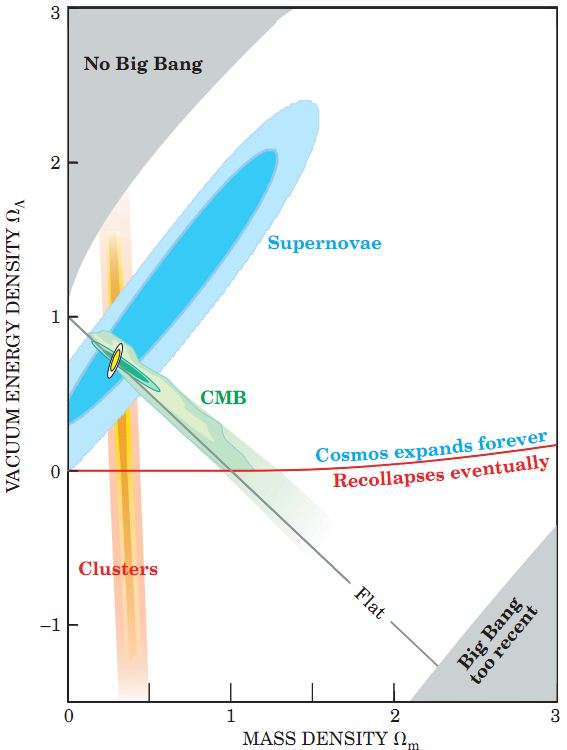
\includegraphics[width=\textwidth]{figure 5.jpg}
    \caption{Values of $\Omega_{\Lambda}$ are plotted against $\Omega_m$ (normalised mass density), along with observations of three phenomena: high red-shift supernovae, CMB and galaxy clusters. The three are shown to converge nicely at $\Omega_m = 0.3$ and $\Omega_{\Lambda} = 0.7$. It can be seen that $\Omega_m+\Omega_{\Lambda} =1$, implying flat geometry. It turns out that a good estimate of the universe's age is also obtained corresponding to these values of density perimeters}
    \label{fig:density}
\end{figure}


%REMEMBER TO CHANGE THE ORDER HERE

\subsection{Age of the Universe}
The cosmological models obtained from the Friedmann equation and the cosmological constant can be used to estimate the age of the universe. The obtain a crude estimate, consider the Hubble parameter. Being the rate of expansion of the universe, it can also be written in the form $r = v H_0^{-1}$, implying that the inverse of it's value is a good timescale to compare the universe age to. Given that the presnt value of the Hubble's constant is estimated to be $H_0 = 100h$ $km s^{-1} Mpc^{-1}$, $H_0^{-1}$ comes out to be $9.77h^{-1}$ x $10^9$ years. This quantity is also called \textbf{Hubble time}. Observation of globular clusters and chemical and thermonuclear activities in stars, as well as obtaining an estimate of the Earth's age, puts the estimated age of the universe between 10-15 billion years. 

A more rigorous calculation can be done by assuming the universe to be matter dominated. This claim is sensible since the a matter dominated universe is more stable, hence this phase can be expected to be present since a considerable time. Hence,

\begin{center}
    $a(t) = (\frac{t}{t_0})^{\frac{2}{3}}$
\end{center}

\begin{center}
    $\implies H = \frac{\dot{a}}{a} = \frac{2}{3t}$
\end{center}

This means that the present time, $t_0 = \frac{2}{3}H_0^{-1}$, which predicts the age as 9.3 billion years, which is incorrect from observations. This value falls further if the universe is assumed to be closed. If the universe is considered open instead and $\Omega_{0}<1$, then the number increases. This is reasonable, since with less matter the amount of gravitational attraction pulling matter inwards would be less and hence it would take the universe a longer time to slow down the expansion rate to the present value. 

Present observations comply nicely with a model in which the universe is flat and density is low, while having a positive cosmological constant. These parameters can be set such that the age exceeds Hubble time:

\begin{equation}
    H_0t_0 = \frac{2}{3}\frac{1}{\sqrt{1-\Omega_0}}ln[\frac{1+\sqrt{1-\Omega_0}}{\sqrt{\Omega_0}}] = \frac{2}{3}\frac{1}{\sqrt{1-\Omega_0}}sinh^{-1}[\sqrt\frac{1-\Omega_0}{\Omega_0}]
\end{equation}

It can be obtained that $t_0 = H_0^{-1}$ when $\Omega_0 = 0.26$. Presently it is estimated that the age of the universe is 14 billion years with $\Omega_0 \approx 0.3$. This is in good agreement with experimental values.

\begin{figure}[H]
    \centering
    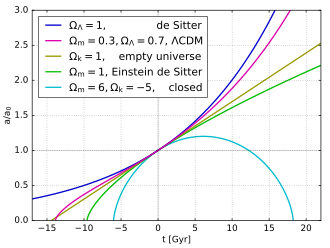
\includegraphics[width=\textwidth]{figure 3.png}
    \caption{Plots which can be used to determine the present age of the universe corresponding to different values of the density parameters. The inclusion of dark matter does alter calculations from those presented in this section.}
    \label{fig:age}
\end{figure}